\documentclass[12pt,letter]{article}
\usepackage[moduleName=Pulses]{KautenjaDSP}
% import a debugging package to show the margin boxes
% \usepackage{showframe}
% set the graphics path to the img directory
\graphicspath{{img/}}

% algorithm2e stuff
% \SetKwInOut{Objects}{$\CKmatrix{O}$}
% \SetKwInOut{Weights}{$\CKvector{w}$}

\begin{document}
\titlePage{Logo}{Module}{KautenjaDSP}

% -------------------
% MARK: Overview
% -------------------

\section{Overview}

Pulses is an emulation of the SunSoft FME7 (5B) sound chip from the Nintendo Entertainment System (NES). The FME7 chip contains three pulse wave generators with level control. Pulses provides the key features of the FME7 chip, namely,
\begin{itemize}
  \item \textbf{Triple pulse wave generator:} Triple pulse waveform generator with duty cycle of $50\%$ and 12-bit frequency value
  \item \textbf{4-bit Amplifier:} A 4-bit amplifier controls the output level of each oscillator with base/attenuator knobs and CV inputs
  \item \textbf{Channel Mixer:} Mix the voices together internally with hard clipping and intentional aliasing
\end{itemize}

% -------------------
% MARK: Panel Layout
% -------------------

\clearpage
\section{Panel Layout}

\begin{figure}[!htp]
\centering
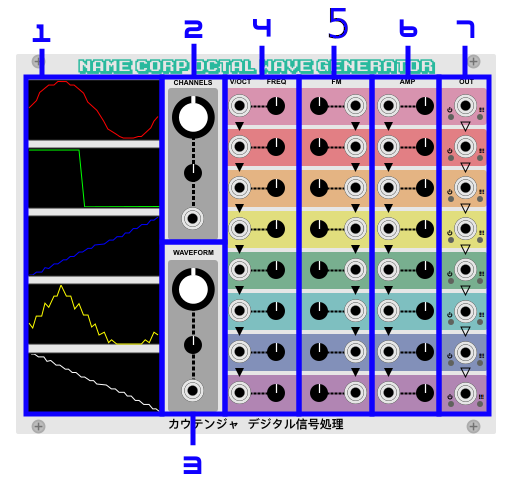
\includegraphics{Interface}
\end{figure}

\subsection*{1{\quad}Frequency}

The trimpot controls the coarse frequency of the three waveform generators. Frequency is quantized to a 12-bit value for the oscillators, which is particularly noticeable in the very low / high registers. The ports provide an exponential $V$/Octave input for controlling the pitch of the tone generators. Inputs are normalled forward from Tone 1, to Tone 2, to Tone 3.

\subsection*{2{\quad}Frequency Modulation}

When nothing is patched to the frequency modulation port, the trimpot can be used to fine tune the frequency of the given waveform generator. When a signal is patched, the input port provides linear frequency modulation to the corresponding waveform generator and the trimpot can be used as an attenuverter to attenuate / polarize the incoming signal. Inputs are normalled forward from Tone 1, to Tone 2, to Tone 3, and support audio rates.

\subsection*{3{\quad}Amplifier}

When no input is connected, the trimpot controls the given waveform generator volume level with 4-bit resolution (i.e., $\in [0, 15]$). When an input is patched to the port, the trimpot acts like an attenuator that scales the CV control over the volume level. Because the amplifier has 4-bit control, the envelope of the voice will sound quantized when used with an external envelope generator. Inputs are normalled forward from Tone 1, to Tone 2, to Tone 3.

\subsection*{4{\quad}Outputs}

Each voice produces an output signal of at most $10V_{pp}$ when the amplifier is maxed out. The individual oscillators cannot be overdriven to produce clipping, distortion, or aliasing. However, outputs are normalled forward into a sum mix where hard clipping \textit{can} occur. Excess clipping will introduce an aliasing effect to the mix. Outputs in the mix are clipped \textit{before} being normalled to the next output. VU meter lights measure the output of individual channels going from off ($-\infty dB$ to $0dB$), to green ($-12dB$ to $0dB$), and lastly to red ($0dB$ to $3dB$) when clipping begins to occur.

% -------------------
% MARK: Data Sheet
% -------------------

\clearpage
\section*{Data Sheet}

\begin{table}[!htp]
\begin{tabular}{|l|l|}
\hline
Type             & Oscillator               \\
\hline
Size             & 8 HP Eurorack            \\
\hline
Depth            & NA                       \\
\hline
Power            & NA                       \\ % 2 x 5 Eurorack
\hline
$+12V$ draw (mA) & 0 mA                     \\
\hline
$-12V$ draw (mA) & 0 mA                     \\
\hline
$+5V$ draw (mA)  & 0 mA                     \\
\hline
Sample Rate      & Programmable             \\
\hline
Bit Depth        & 16-bit                   \\
\hline
\end{tabular}
\end{table}

% -------------------
% MARK: References
% -------------------

\clearpage
\renewcommand\refname{References \& Acknowledgments}
\nocite{*}
\bibliographystyle{apalike}
\bibliography{references}

\end{document}
